\section{单项选择题}
\begin{enumerate}
	\item 与向量$\vec{a}=(1,-1,0)$及向量$\vec{b}=(1,0,-2)$同时垂直的单位向量为\emptychoice
		\begin{choice}(4)
			\choice $(1,2,2)$
			\choice $(\frac{2}{3},\frac{2}{3},\frac{1}{3})$
			\choice $(2,2,1)$
			\choice $(\frac{1}{3},\frac{2}{3},\frac{1}{3})$
		\end{choice}
	\item 下列各组角中,可以作为向量的方向角的是\emptychoice
		\begin{choice}(4)
			\choice $\frac{\pi}{3},\frac{\pi}{4},\frac{2\pi}{3} $
			\choice $-\frac{\pi}{3},\frac{\pi}{4},\frac{\pi}{3} $
			\choice $\frac{\pi}{6},\pi,\frac{\pi}{6} $
			\choice $\frac{2\pi}{3},\frac{\pi}{3},\frac{\pi}{3} $
		\end{choice}
	\item 平面$x-2y+z+1=0$与下列平面\emptychoice 垂直.
		\begin{choice}(4)
			\choice $-x+2y-z-5=0$
			\choice $2x-y+3z+5=0$
			\choice $-x+y+3z-10=0$
			\choice $3x-5y+z+4=0$
		\end{choice}
	\item 直线$ \frac{x-1}{3}=\frac{y+1}{-1}=\frac{z-2}{1} $与平面$ x+2y-z+3=0 $的位置关系是\emptychoice
		\begin{choice}(2)
			\choice 互相垂直
			\choice 互相平行但直线不在平面上
			\choice 即不平行也不垂直
			\choice 直线在平面上
		\end{choice}
	\item 已知$ \vec{a}=(-1,1,2), \vec{b}=(2,0,1) $,则向量$ \vec{a} $与$ \vec{b} $的夹角为\emptychoice
		\begin{choice}(4)
			\choice 0
			\choice $ \frac{\pi}{6} $
			\choice $ \frac{\pi}{4} $
			\choice $ \frac{\pi}{2} $
		\end{choice}
	\item 直线$ \frac{x-1}{-1}=\frac{y-2}{2}=\frac{z+1}{-2} $与下列平面\emptychoice 平行.
		\begin{choice}(2)
			\choice $ 4x+y-z+10=0 $
			\choice $ x-2y+3z+5 $
			\choice $ 2x-3y+z+6 $
			\choice $ -x-y+5z+4=0 $
		\end{choice}
\end{enumerate}
\section{填空题}
\begin{enumerate}
	\item 向量$\vec{a}=-2\vec{i}+3\vec{j}-\vec{k}$与$\vec{b}=m\vec{i}-2\vec{k}$垂直,则$m=$\blank .
	\item 点$(-1,6,2)$关于$y$轴对称点的坐标为\blank .
	\item 向量$\vec{a}=(-2,6,-3)$的模为$ |\vec{a}|= $\blank ,与$ \vec{a} $同向的单位向量$ \vec{e}= $\blank .
	\item 设$\alpha,\beta,\gamma$是向量$\vec{a}$的三个方向角,则$ \sin^2 \alpha + \sin^2 \beta + \sin^2 \gamma = $\blank .
	\item 空间两点$ A(2,1,1) $与$ B(-1,0,3) $的距离为\blank .
	\item 直线$ \frac{x-1}{m}=\frac{y+2}{2}=\frac{z-5}{-1}$与平面$ x-2y+3z-1=0 $平行,则$m=$\blank .
	\item 平面曲线$ \frac{y^2}{b^2}+\frac{z^2}{c^2}=1 $绕$ y $轴旋转所得到的空间曲面为\blank .
	\item 两非零向量$ \vec{a} $与$ \vec{b} $垂直的充要条件是\blank ,两非零向量$ \vec{a} $与$ \vec{b} $平行的充要条件是\blank .
	\item 点(1,2,1)到平面$ x+2y+2z-10=0 $的距离为\blank .
	\item 已知两点$ M_1(0,1,2) $和$ M_2(1,-1,0) $,则$ -2\overrightarrow{M_1M_2}=$\blank .
	\item 向量的终点为(2,-1,7),它在$ x,y,z $坐标轴上的投影分别为4,-4,7,则起点为\blank .
	\item 向量$ \vec{a}=(4,-3,4) $在向量$ \vec{b}=(2,2,1) $上的投影为\blank .
	\item 平面$ 2x-4y-z+4=0 $在$ x,y,z $三个坐标轴上的截距依次为\blank[1em],\blank[1em],\blank[1em].
\end{enumerate}
\section{计算题}
\begin{enumerate}
	\item 求到两点$ M(3,-5,2) $和$ N(4,-1,7) $距离相等的点的轨迹方程.
	\item 求与坐标原点$ O $及点(2,3,4)的距离之比为1:2的点的全体组成的曲面的面积,它表示怎样的曲面?
	\item 设$ \vec{a}=(1,3,-1),\vec{b}=(-1,1,0) $,求:
		\begin{enumerate}[(1)]
			\item $\vec{a}\cdot\vec{b}$及$\vec{a}$与$\vec{b}$的夹角;
			\item $ \vec{a}\times\vec{b} $及同时垂直于$ \vec{a},\vec{b} $的单位向量;
			\item 以$\vec{a},\vec{b}$为三角形的两边所构成的三角形的面积.
		\end{enumerate}
	\item 求过(1,1,-1),(-2,-2,2)和(1,-1,2)三点的平面方程.
	\item 求通过$ z $轴和点(-3,1,-2)的平面方程.
	\item 已知两条直线的方程是$ l_1:\frac{x-1}{1}=\frac{y-2}{0}=\frac{z-3}{-1} $,$ l_2:\frac{x+2}{2}=\frac{y-1}{1}=\frac{z}{1} $,求通过$ l_1 $且平行于$ l_2 $的平面方程.
	\item 求过$ M_1(3,-2,1) $和$ M_2(-1,0,2) $两点的直线方程.
	\item 求过点(4,-1,3)且平行于直线$ \frac{x-3}{2}=\frac{y}{1}=\frac{z-1}{5} $的直线方程.
	\item 求直线$ \begin{cases} 5x-3y+3z-9=0 \\ 3x-2y+z-1=0 \end{cases} $与直线$ \begin{cases} 2x+2y-z+23=0 \\ 3x+8y+z-18=0 \end{cases} $的夹角的余弦.
	\item 求点$ P(3,-1,2) $到直线$ \begin{cases} x+y-z+1=0 \\ 2x-y+z-4=0 \end{cases} $的距离.
\end{enumerate}
\section{证明题}
\begin{enumerate}
	\item 如果平面上一个四边形的对角线互相平分,则它为一平行四边形.
	\item 直径所对的圆周角为直角.
\end{enumerate}
\section{单项选择题解答}
\begin{enumerate}
	\item B\\
		解析:两向量垂直等价于数量积为0,只需分别计算4个选项中哪一项与$ \vec{a} $和$ \vec{b} $数量积均为0.
	\item A\\
		解析:方向角在$[0,\pi]$之间,且满足3者的余弦平方和为1.
	\item C\\
		解析:两个相互垂直的平面的法向量也相互垂直. 题目所给平面法向量是$ (1,-2,1) $,C选项法向量是$ (-1,1, 3) $,它们的数量积为0.
	\item D\\
		解析:直线方向向量是$\vec{s}=(3,-1,1)$,平面法向量是$ \vec{n}=(1,2,-1) $. 它们的数量积为0. 所以两向量垂直,即直线与平面平行或位于平面上. 从直线方程可知直线过点$ (1,-1,2) $,将该点代入平面方程发现它也满足平面方程,所以直线在平面上.
	\item D\\
		解析:用夹角余弦公式$ \cos{\theta}=\frac{\vec{a}\cdot\vec{b}}{|\vec{a}||\vec{b}|} $计算出夹角余弦是0. 所以夹角是$ \frac{\pi}{2} $.
	\item A\\
		解析:直线与平面平行,则直线的方向向量与平面的法向量垂直. 直线的方向向量是$ (-1,2,-2) $,A选项平面的法向量是$ (4,1,-1) $,它们是数量积为0.
\end{enumerate}
\section{填空题解答}
\begin{enumerate}
	\item 1\\
		解析:$ \vec{a}\cdot\vec{b} = -2m+2 = 0 $,得$ m=1 $.
	\item $(1,6,-2)$\\
		解析:将$ y $坐标保持不变,$ x,z $坐标变为原来的相反数.
	\item $7$;$ (-\frac{2}{7},\frac{6}{7},-\frac{3}{7}) $\\
		解析:$ |\vec{a}|=\sqrt{(-2)^2+6^2+(-3)^2}=7 $, $ \vec{e}=\frac{\vec{a}}{7} $.
	\item $2$\\
		解析:$ \sin^2 \alpha + \sin^2 \beta + \sin^2 \gamma = 1-\cos^2 \alpha + 1-\cos^2 \beta + 1-\cos^2 \gamma = 3 - (\cos^2 \alpha + \cos^2 \beta + \cos^2 \gamma) = 3-1 = 2$.
	\item $ \sqrt{14} $\\
		解析:$ |AB|=\sqrt{3^2+1^2+(-2)^2}=\sqrt{14} $.
	\item 7\\
		解析:直线与平面平行,则直线的方向向量与平面的法向量垂直,所以$ (m,2,-1)\cdot(1,-2,3)=m-4-3=0\Rightarrow m = 7 $.
	\item $ \frac{y^2}{b^2}+\frac{x^2+z^2}{c^2}=1 $\\
		解析:绕$ y $轴旋转,则$ y $坐标不发生变化,所以$ z $坐标变为$ \pm\sqrt{x^2+z^2} $. 旋转后的曲面为椭球面.
	\item $ \vec{a}\cdot\vec{b}=0 $;存在唯一实数$ \lambda $使得$ \vec{a}=\lambda\vec{b} $\\
		解析:见课本第5页定理1和第15页数量积的性质(2).
	\item 1\\
		解析:令$ f(x,y,z)=x+2y+2z-10 $,则点到平面的距离为$ \frac{|f(1,2,1)|}{\sqrt{1+4+4}}=1 $.
	\item (-2,4,4)\\
		解析:$ M_2 $点坐标减去$ M_1 $点坐标得$ \overrightarrow{M_1M_2}=(1,-2,-2) $,再乘以-2可得答案$ (-2,4,4) $.
	\item (-2,3,0)\\
		解析:该向量的坐标形式为$ (4,-4,7) $,其起点坐标=终点坐标-向量坐标=$ (-2,3,0) $.
	\item 2\\
		解析:$ \Prj_{\vec{b}}\vec{a} = |\vec{a}|\cos(\widehat{\vec{a},\vec{b}}) = \frac{\vec{a}\cdot\vec{b}}{|\vec{b}|} = 2 $.
	\item -2;1;4\\
		解析:分别令$ y,z $、$ x,z $、$ x,y $坐标为0计算另一坐标,可得在$ x,y,z $三个坐标轴上的截距依次为-2,1,4.
\end{enumerate}
\section{计算题解答}
\begin{enumerate}
	\item 解:列方程可得\[ \begin{split}
(x-3)^2+(y+5)^2+(z-2)^2 &= (x-4)^2+(y+1)^2+(z-7)^2 \\
-6x+9+10y+25-4z+4 &= -8x+16+2y+1-14z+49 \\
2x+8y+10z-28 & = 0 \\
x+4y+5z-14 & = 0
\end{split} \]
	\item 解:由$$
\frac{\sqrt{x^2+y^2+z^2}}{\sqrt{(x-2)^2+(y-3)^2+(z-4)^2}}=\frac{1}{2}
$$得$$
(x+\frac{1}{3})^2+(y+1)^2+(z+\frac{4}{3})^2 = \frac{104}{9}
$$
所以该曲面是球心在$ (-\frac{1}{3},-1,-\frac{4}{3}) $,半径为$ \frac{2\sqrt{26}}{3} $的球.\\
面积为$ 4\pi\cdot\frac{104}{9}=\frac{416}{9}\pi $.
	\item 解:
		\begin{enumerate}[(1)]
			\item $ \vec{a}\cdot\vec{b}=-1+3+0=2 $. $ \cos(\widehat{\vec{a},\vec{b}})=\frac{\vec{a}\cdot\vec{b}}{|\vec{a}||\vec{b}|}=\frac{\sqrt{22}}{11} $,所以夹角$ (\widehat{\vec{a},\vec{b}})=\arccos\frac{\sqrt{22}}{11} $.
			\item $ \vec{a}\times\vec{b}=\left| \begin{matrix}
	\vec{i}&		\vec{j}&		\vec{k}\\
													1&		3&		-1\\
													-1&		1&		0\\
												\end{matrix} \right| = \vec{i}+\vec{j}+4\vec{k}=(1,1,4) $,垂直于$ \vec{a},\vec{b} $的单位向量为$ \frac{\vec{a}\times\vec{b}}{|\vec{a}\times\vec{b}|}=(\frac{\sqrt{2}}{6},\frac{\sqrt{2}}{6},\frac{2\sqrt{2}}{3}) $.
			\item 面积$ s=\frac{1}{2}|\vec{a}\times\vec{b}|=\frac{3\sqrt{2}}{2} $.
		\end{enumerate}
	\item 解:令$ \vec{a}=(-2,-2,2)-(1,1,-1)=(-3,-3,3) $,$ \vec{b}=(1,1,-1)-(1,-1,2)=(0,2,-3) $,则平面法向量$ \vec{n}=\vec{a}\times\vec{b}=(3,-9,-6) $.\\
平面方程为$ 3(x-1)-9(y-1)-6(z+1)=0 $,化简得$ x-3y-2z=0 $.
	\item 解:令$ \vec{a}=(0,0,1) $,$ b=-3,1,-2 $,则平面法向量$ \vec{n}=\vec{a}\times\vec{b}=(-1,-3,0) $,又平面过原点$ (0,0,0) $,故平面方程为$ -x-3y=0 $,或$ x+3y=0 $.
	\item 解:设$ \vec{a} $为直线$ l_1 $的方向向量,$ \vec{b} $为直线$ l_2 $的方向向量,则$ \vec{a}=(1,-0,-1) $,$ \vec{b}=(2,1,1) $.\\
平面法向量为$ \vec{n}=\vec{a}\times\vec{b}=(1,-3,1) $. 点$ (1,2,3) $在直线$ l_1 $上,故也在要求的平面上.\\
所以平面方程为$ (x-1)-3(y-2)+(z-3)=0 $,化简得$ x-3y+z+2=0 $.
	\item 解:方向向量$ \vec{s}=(4,-2,-1) $,点向式方程为$ \frac{x-3}{4}=\frac{y+2}{-2}=\frac{z-1}{-1} $.
	\item 解:方向向量$ \vec{s}=(2,1,5) $,点向式方程为$ \frac{x-4}{2}=\frac{y+1}{1}=\frac{z-3}{5} $.
	\item 解:设$ \vec{s_1},\vec{s_2} $为两直线方向向量,$ \theta $为两直线夹角.则$ \vec{s_1}=(5,-3,3)\times(3,-2,1)=(3,4,-1) $,$ \vec{s_2}=(2,2,-1)\times(3,8,1)=5(2,-1,2) $,只考虑方向的话可令$ \vec{s_2}=(2,-1,2) $.\\
计算得两直线夹角的余弦为$ \cos\theta = \frac{\vec{s_1}\cdot\vec{s_2}}{|\vec{s_1}||\vec{s_2}|}=0 $.
	\item 解:设$ \vec{s} $为直线的方向向量,则$ \vec{s}=(1,1,-1)\times(2,-1,1)=(0,-3,-3) $.\\
过点$ P $垂直于直线的平面为$ y+z-1=0 $.\\
该平面与直线的交点为方程组$$ \begin{cases}
x+y-z+1=0 \\
2x-y+z-4=0 \\
y+z-1 =0
\end{cases} $$的解,其解为$ (1,-\frac{1}{2},\frac{3}{2}) $.\\
所以点$ P $到直线的距离为$ \sqrt{(3-1)^2+(-1+\frac{1}{2})^2+(2-\frac{3}{2})^2}=\frac{3\sqrt{2}}{2} $.
\end{enumerate}
\section{证明题解答}
\begin{enumerate}
	\item 证明:\begin{minipage}[t]{0.6\linewidth}
		已知$ \overrightarrow{CO} = \overrightarrow{OB} $,$ \overrightarrow{AO}=\overrightarrow{OD} $,则有$ \overrightarrow{CD}=\overrightarrow{CO}+\overrightarrow{OD}=\overrightarrow{OB}+\overrightarrow{AO}=\overrightarrow{AB} $.
		同理,$ \overrightarrow{AC}=\overrightarrow{BD} $. 所以该四边形对边相互平行,它是平行四边形.
	\end{minipage}
	\begin{minipage}[t]{0.3\linewidth}\strut\vspace*{-\baselineskip}\newline
		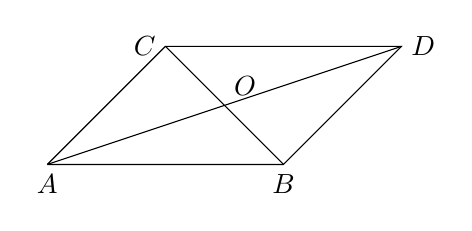
\begin{tikzpicture}[scale=1.5]
		\draw[] (0,0) node[below]{$A$} -- (2,0) node[below]{$B$} -- (3,1) node[right]{$D$} -- (1,1) node[left]{$C$} -- (0,0);
		\draw[] (0,0) -- (3,1);
		\draw[] (1,1) -- (2,0);
		\draw[] (3/2,1/2) node[above right]{$O$};
		\end{tikzpicture}
	\end{minipage}
	\item 证明:\begin{minipage}[t]{0.6\linewidth}
		如图,$ \overrightarrow{OA} = -\overrightarrow{OB} $,$ |\overrightarrow{OA}|=|\overrightarrow{OB}|=|\overrightarrow{OC}| $,且$ \overrightarrow{CA}=\overrightarrow{CO}+\overrightarrow{OA} $,$ \overrightarrow{CB}=\overrightarrow{CO}=\overrightarrow{OB} $.
		
		所以,$ \overrightarrow{CA}\cdot\overrightarrow{CB} = (\overrightarrow{CO}+\overrightarrow{OA})\cdot(\overrightarrow{CO}=\overrightarrow{OB})=|\overrightarrow{CO}|^2 + \overrightarrow{CO}\cdot\overrightarrow{OB} - \overrightarrow{CO}\cdot\overrightarrow{OB} - |\overrightarrow{CO}|^2 = 0$. 所以$ \overrightarrow{CA}\perp\overrightarrow{CB} $,即直径所对的圆周角为直角.
	\end{minipage}
	\begin{minipage}[t]{0.3\linewidth}\strut\vspace*{-\baselineskip}\newline
		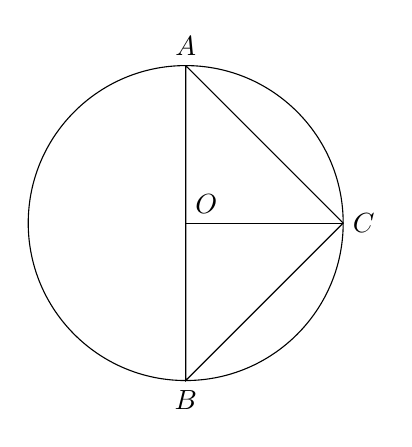
\begin{tikzpicture}[scale=1]
		\draw[] (0,0) circle (2);
		\draw[] (0,2) node[above]{$A$} -- (0,-2) node[below]{$B$} -- (2,0) node[right]{$C$} -- (0,2);
		\draw[] (0,0) node[above right]{$O$} -- (2,0);
		\end{tikzpicture}
	\end{minipage}
\end{enumerate}
